\chapter{Chain conformation analysis}\label{chap_analysis}
\graphicspath{{./analysis/graphs/}}

\section{Polymer crystallization}

\subsection{Polymer crystal models and theories}

Material systems naturally tend to stay in a lower energy state. Therefore a regular liquid upon cooling transition into solid state (the ground state), with either amorphous or crystalline state. For a polymer, the chains are entangled and aligned in all directions in liquid state, so it is much more difficult to achieve its ground state, with the monomers sitting on crystal lattice points and the chains aligned perfectly parallel with each other. However, polymers could still crystallize under proper conditions, adopting a more complex structure rather than the ideal crystalline state, and this process does not only depend on thermodynamics, but kinetics as well.

Before we look at long polymers chains, oligomers (especially linear ones) are a simpler yet close enough example in terms of crystallization. Based on X-ray crystallography results, oligomer crystals adopt a structure of stacked layers, with each layer composed of chains standing up perpendicular to the layer surface (Figure \ref{fig:oligomercrystallization}). Among neighboring layers, end-groups of the chains form the amorphous phase at the interfaces (not shown in the drawing) \cite{Strobl2007}.

\begin{figure}[H]
\center
\vspace{1 cm}
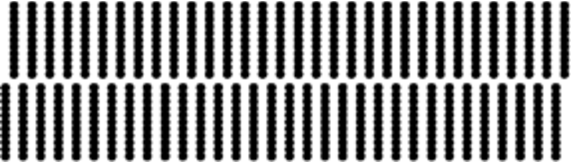
\includegraphics[width=0.7\linewidth]{oligomercrystallization}
\caption[Oligomer crystal structure.]{Oligomer crystal structure \cite{Strobl2007}.}
\label{fig:oligomercrystallization}
\end{figure}

For crystallization of polymers with higher molecular weights, however, it is impossible for the chains to completely disentangle, which requires an extremely high energy and a very long time. Limited by the nature of polymers themselves, the chains align into local crystalline domains, with some unresolved entanglements left as amorphous phases in between. Similar to oligomers, end-groups are also part of the amorphous phase. Therefore, polymer crystals are called semicrystalline crystals.

\subsubsection{Fringed micelle model}

In order to describe semicrystalline polymer crystal structures in further details, different models and theories have been proposed. One of the earliest models is fringed micelle model \cite{HerrmannKGerngrossO1930}. In this model, both the crystalline phase and the amorphous phase are present, with the crystallites existing as local domains. The micelles of crystalline parts have sizes much smaller than the chain lengths, so a single polymer chain is believed to be able to pass through several micelles, thus binding them together.

%Herrmann, K.; Gerngross, O.; Abitz, W. Zur rontgenographischen Strukturforschung des gelatinemicells. Z. Phys. Chem. B 1930, 10, 371–394.

\begin{figure}[H]
\center
\vspace{1 cm}
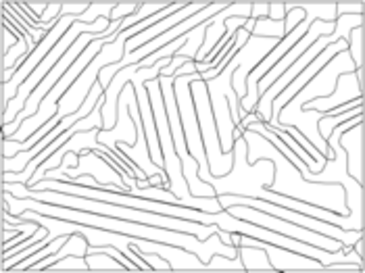
\includegraphics[width=0.4\linewidth]{fringedmicelle}
\caption[Fringed micelle model of polymer crystal structure.]{Fringed micelle model of polymer crystal structure \cite{Flory1953}.}
\label{fig:fringedmicelle}
\end{figure}

However, there were some problems with fringed micelle model. According to the calculation of free energy, it was found that there would be a large conformational entropy loss for the amorphous chains if this model was true \cite{Flory1962}. In addition, experimentalists observed evidences of large crystallites - "sperulites", which have a strong preference in terms of the alignment of chains, and are highly symmetrical instead of a random distribution of crystallites \cite{Geil1964}. Together with some other flaws and contradictions found with the model itself \cite{Zachmann1967,Zachmann1969}, people began to doubt fringed micelle model and try to find other ways to describe semicrystalline polymer crystals.

\subsubsection{Folded chain model} \label{folded chain model}

As the fringed micelle model was being questioned, some crucial experimetal observations led to the birth of a new model of polymer crystals---the folded chain model. The concept of chain-folding was actually first proposed by Storks \cite{Storks1938}. He observed unstretched films of gutta-percha through electron diffraction measurements, and found that the films are composed of large crystallites with the chain axis perpendicular to the film surfaces. The thickness of the films are much smaller than the chain lengths, which led to Storks' proposal that the chains need to fold themselves inside the film.  At that time, fringed micelle model was still dominating the directions of polymer crystallization researches, so his results and proposal did not receive much attention. Later, several researchers \cite{JACCODINE1955,Till1957,Keller1957} studied polymer single crystals and found that they have smooth surfaces, with heights of about 10 nm, which is also much smaller than the chain lengths. The chains are believed to fold themselves back and forth in each lamella, and when the polymer solution concentration is high enough, or when the polymer crystallizes from a melt, mutiple lamellae stack together to form a crystal. These observations helped the development of folded chain model, which from then on became the most widely accepted model of polymer crystals. 

Now it is clear that the chains fold in crystal, and next step would be to determine the way of chain folding. After the chain gets to the amorphous interface and fold itself back, it is not clear where it re-enters the lamella. There have been a large number of studies on this \cite{Kovacs1975,Yoon1979,Keller1979} and two major models have been proposed: adjacent re-entry model and random re-entry model.

As adjacent re-entry model describes, after a chain escapes the lamella and makes a fold, it turns right back and inserts into the neighboring site. In this way, the lamellae created have relatively smooth surfaces, as Figure \ref{fig:adjacent} shows.

\begin{figure}[H]
\center
\vspace{1 cm}
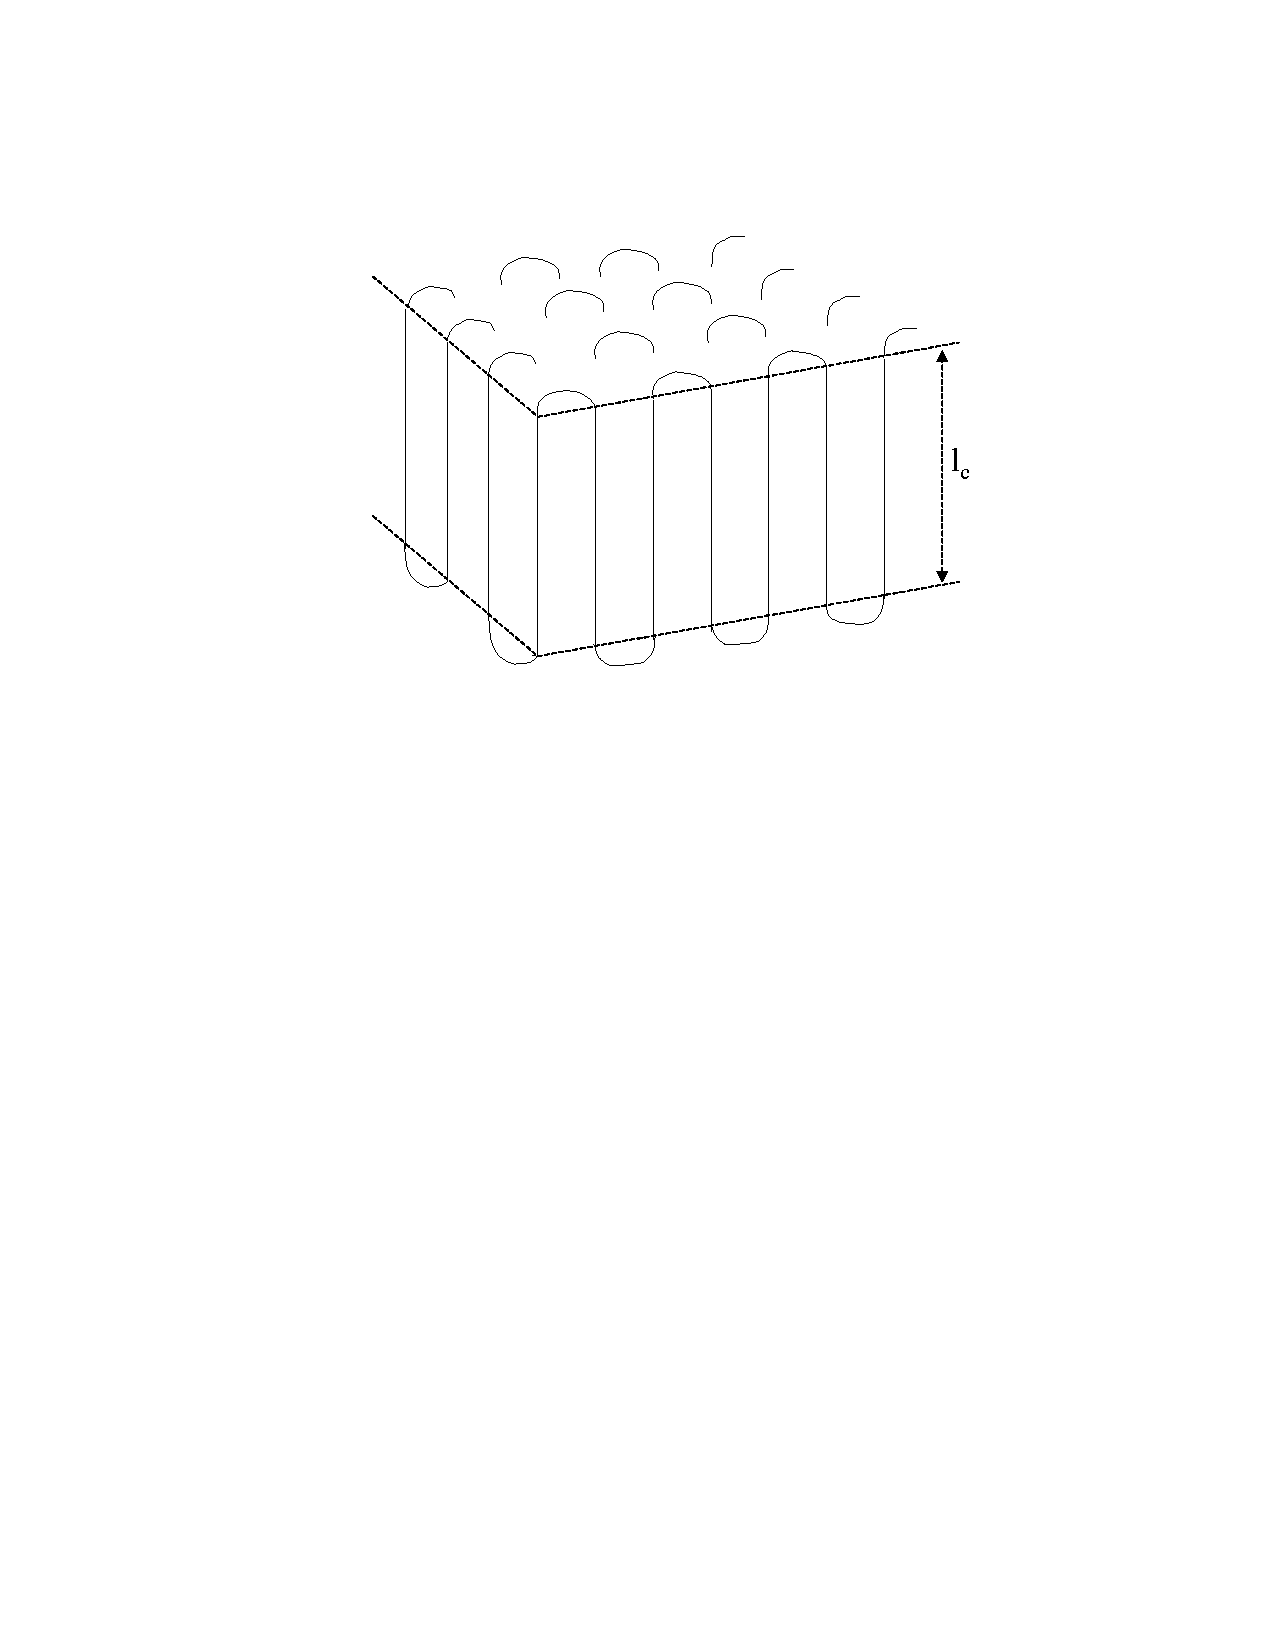
\includegraphics[width=0.4\linewidth]{adjacent}
\caption[Adjacent re-entry model of polymer crystals.]{Adjacent re-entry model of polymer crystals \cite{High}.}
\label{fig:adjacent}
\end{figure}

Random re-entry model is also known as switchboard model. Instead of folding right back into the neighboring site on the same lamella, a chain that emanated from the lamellar surface could either float on the interface and walk into a further site, or even enters a neighboring lamella, which leads to a completely random arrangement on the interfaces of lamellae and amorphous regions (Figure \ref{fig:random}).

\begin{figure}[H]
\center
\vspace{1 cm}
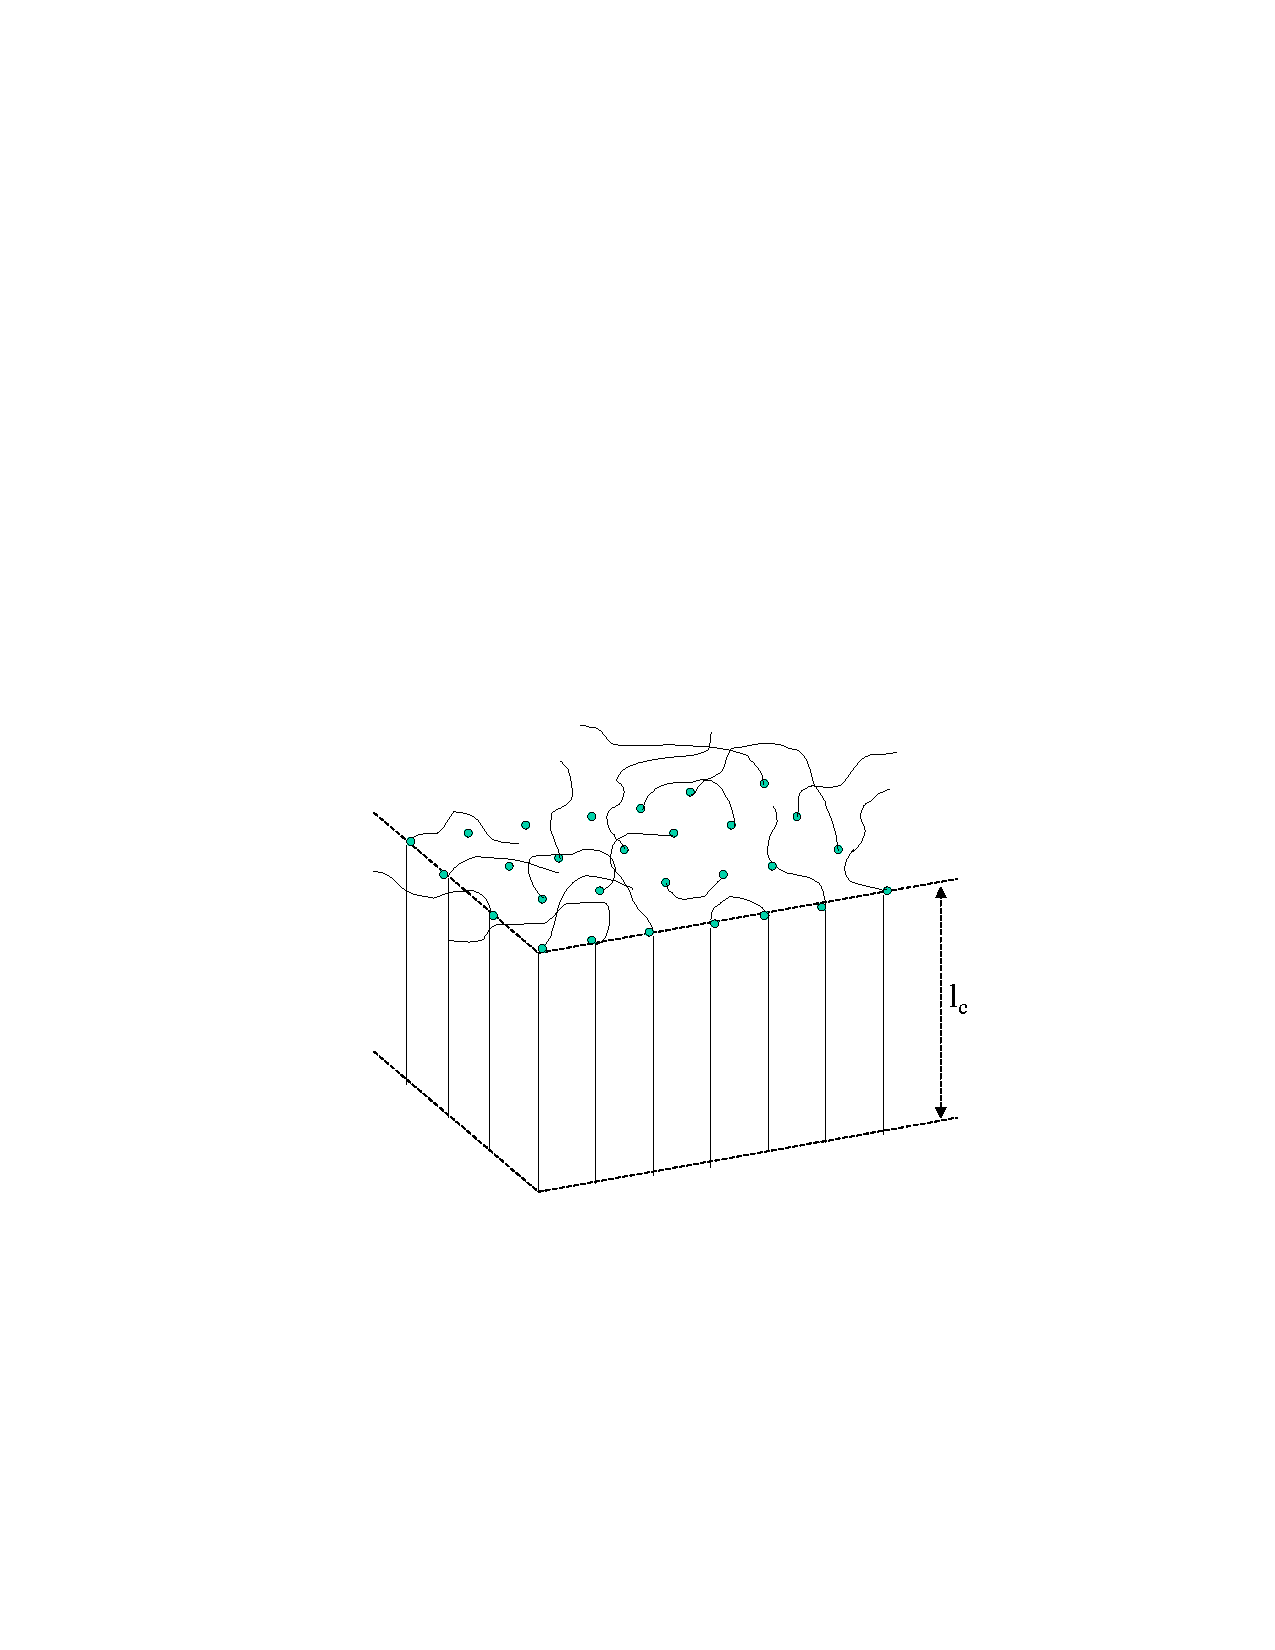
\includegraphics[width=0.4\linewidth]{random}
\caption[Random re-entry model of polymer crystals.]{Random re-entry model of polymer crystals \cite{High}.}
\label{fig:random}
\end{figure}

Adjacent re-entry model would result in a much more thermodynamically favorable conformation with a lower entropy. However, in a real situation of polymer crystallization, twisting, misalignment, and entanglements of the long chains prevent them from relaxing and aligning perfectly in regular folds. Instead, regions consisting too many entanglements are more likely to be shifted to the surfaces and contribute to the amorphous phase \cite{Strobl2007}. Taking both thermodynamics and kinetics factors into account, real polymer crystal lamellae are normally composed of both adjacent re-entries and random re-entries. It should be noted that in real cases, chain-folding also depends on more factors: chain lengths, flexibility of chains, crystallization temperature, cooling rate, chain defects, etc.
 
\subsection{Thermodynamics of polymer crystallization} \label{Thermodynamics of polymer crystallization}

Thermodynamics is the fundamental rule that polymer chains obey during crystallization. The most favorable state for polymers is that with the lowest possible free energy $G$. $G$ is lower for melt than for crystals at high temperatures, while it is lower for crystals than for melt at low temperatures. The equilibrium melting point $T_{m}^{\infty}$ is defined as the temperature at which the liquid state and the solid state have the same free energy. Therefore, the change in Gibbs free energy, $\Delta G$, is equal to zero during melting or crystallization transition at thermodynamic equilibrium:

\begin{equation}
\label{eqn_deltaG}
\Delta G = \Delta H - T_{m}^{\infty} \Delta S = 0
\end{equation}

\begin{equation}
\label{eqn_Tminfinity}
T_{m}^{\infty} = \dfrac{\Delta H}{\Delta S}
\end{equation}

In practical cases, the crystallization temperature $T_{c}$ is always lower than the melting temperature $T_{m}$, and their difference is defined as the supercooling $\Delta T$. This is mainly due to the nucleation and growth mechanism during crystallization. A nucleus must be present to initialize the growth of a crystal, and when there is no present nuclei, the temperature needs to keep decreasing until the melt itself starts a primary nucleation. This mechanism will also be further discussed in Chapter \ref{chap_growth}. Compared to regular crystals, $\Delta T$ of polymers could be as large as 20 to 30 K, resulting from the metastable chain-folding nature of polymers \cite{Hu2013}.

Equation \ref{eqn_Tminfinity} tells us that the equilibrium melting temperature depends on both enthalpy and entropy of the system. However, the effect of surface energy and crystal size has not been considered. For a real polymer crystal, shape and size of the lamella would directly affect its melting point, and this effect could be examined through thermodynamics.

Let us start with an infinitely large crystal, and from conventional thermodynamic viewpoints it is considered not to involve surface energy. Therefore its melting point is believed to be $T_{m}^{\infty}$.

Now assume a lamella with length $a$, width $b$, and height $l$, where $a \gg l$, and $b \gg l$. The surface energy per unit area of the top and bottom surfaces is $\sigma_{e}$, and the surface energy per unit area of the side surfaces is $\sigma$. This lamella with the finite size effect could be considered as a quasi-two dimensional object with one-dimensional confinement \cite{Zhang2016}. The free energy per unit mass on melting is $\Delta g$, and the total free energy $\Delta G$ on melting consists of the energy required to create new surfaces and the energy of fusion for the bulk:

\begin{equation}
\label{eqn_delta G lamella}
\Delta G = 2(a+b)l\sigma + 2ab\sigma_{e} - abl\Delta g
\end{equation}

\noindent
and with $\sigma_{e}\gg\sigma$, $a\gg l$, $b\gg l$, the total free energy is then:

\begin{equation}
\label{eqn_delta G lamella reduced}
\Delta G = 2ab\sigma_{e} - abl\Delta g
\end{equation}

At melting temperature $T_{m}$, $\Delta G = 0$, which leads to:

\begin{equation}
\label{eqn_delta g lamella}
\Delta g (T_{m}) = \dfrac{2\sigma_{e}}{l}
\end{equation}

Once again, for an infinitely large crystal, we have:

\begin{equation}
\label{eqn_delta g large}
\Delta g (T_{m}^{\infty}) = \Delta h (T_{m}^{\infty}) - T_{m}^{\infty}\Delta s (T_{m}^{\infty}) = 0
\end{equation}

Assuming between $T_{m}$ and $T_{m}^{\infty}$, the enthalpy and entropy could be treated as invariant, we further have:

\begin{equation}
\label{eqn_delta g}
\Delta g (T_{m}) = \Delta h (T_{m}) - T_{m}\Delta s (T_{m})
\end{equation}

Combining Equation \ref{eqn_delta g large} and Equation \ref{eqn_delta g}, we are able to generate:

\begin{equation}
\label{eqn_delta g 2}
\Delta g (T_{m}) = \Delta h (T_{m}) - T_{m}\dfrac{\Delta h (T_{m})}{T_{m}^{\infty}}
\end{equation}

Now with Equation \ref{eqn_delta g lamella} and Equation \ref{eqn_delta g 2}, we finally obtain the relation between the thickness of a lamella and its melting temperature:

\begin{equation}
\label{eqn_GT}
T_{m} = T_{m}^{\infty} (1 - \dfrac{2\sigma_{e}}{l \Delta h})
\end{equation}

\noindent
which is the well-known Gibbs Thomson equation. It has been applied to many polymers with linear structure and has proved to provide reliable predictions of the melting temperature as a function of lamella thickness \cite{KojiYamada2003}. With a larger thickness, the finite size effect is weaker, and the melting temperature $T_{m}$ of the lamella would be closer to the equilibrium melting temperature $T_{m}^{\infty}$.

\section{PEO crystallization}

In terms of crystallization, PEO is one of the most intensively studied polymers, together with Poly(Ethylene) and n-alkanes. With a linear structure, these polymers all crystallize very easily. As a semicrystalline polymer, PEO chains fold into lamellar structures during crystallization process, and multiple lamellae stack up to form the whole crystal \cite{Arlif1966}. In our case, we focus on low molecular weight PEO, so crystallization should be even easier since the chains are relatively short and thus need fewer times of folding. When the number of folds changes, the thickness of the lamella varies, which has a direct influence on the melting temperature of the crystal lamella.

\subsection{Crystal structure}

PEO crystals have monoclinic unit cells, with the chains adopting a structure of 7/2 helix with trans-gauche-trans conformation. In this conformation, seven monomeric units form two periods of the helix, which is 1.93 nm long \cite{Yoshihara1964}. As shown in Figure \ref{fig:PEOhelix}, every bond is rotated by a certain angle with respect to the c-axis (vertical axis) of the lamella, and the projection length of one monomer on the c-axis, $l_{c}$, is 0.278 nm \cite{Takahashi1973}.

\begin{figure}[H]
\center
\vspace{1 cm}
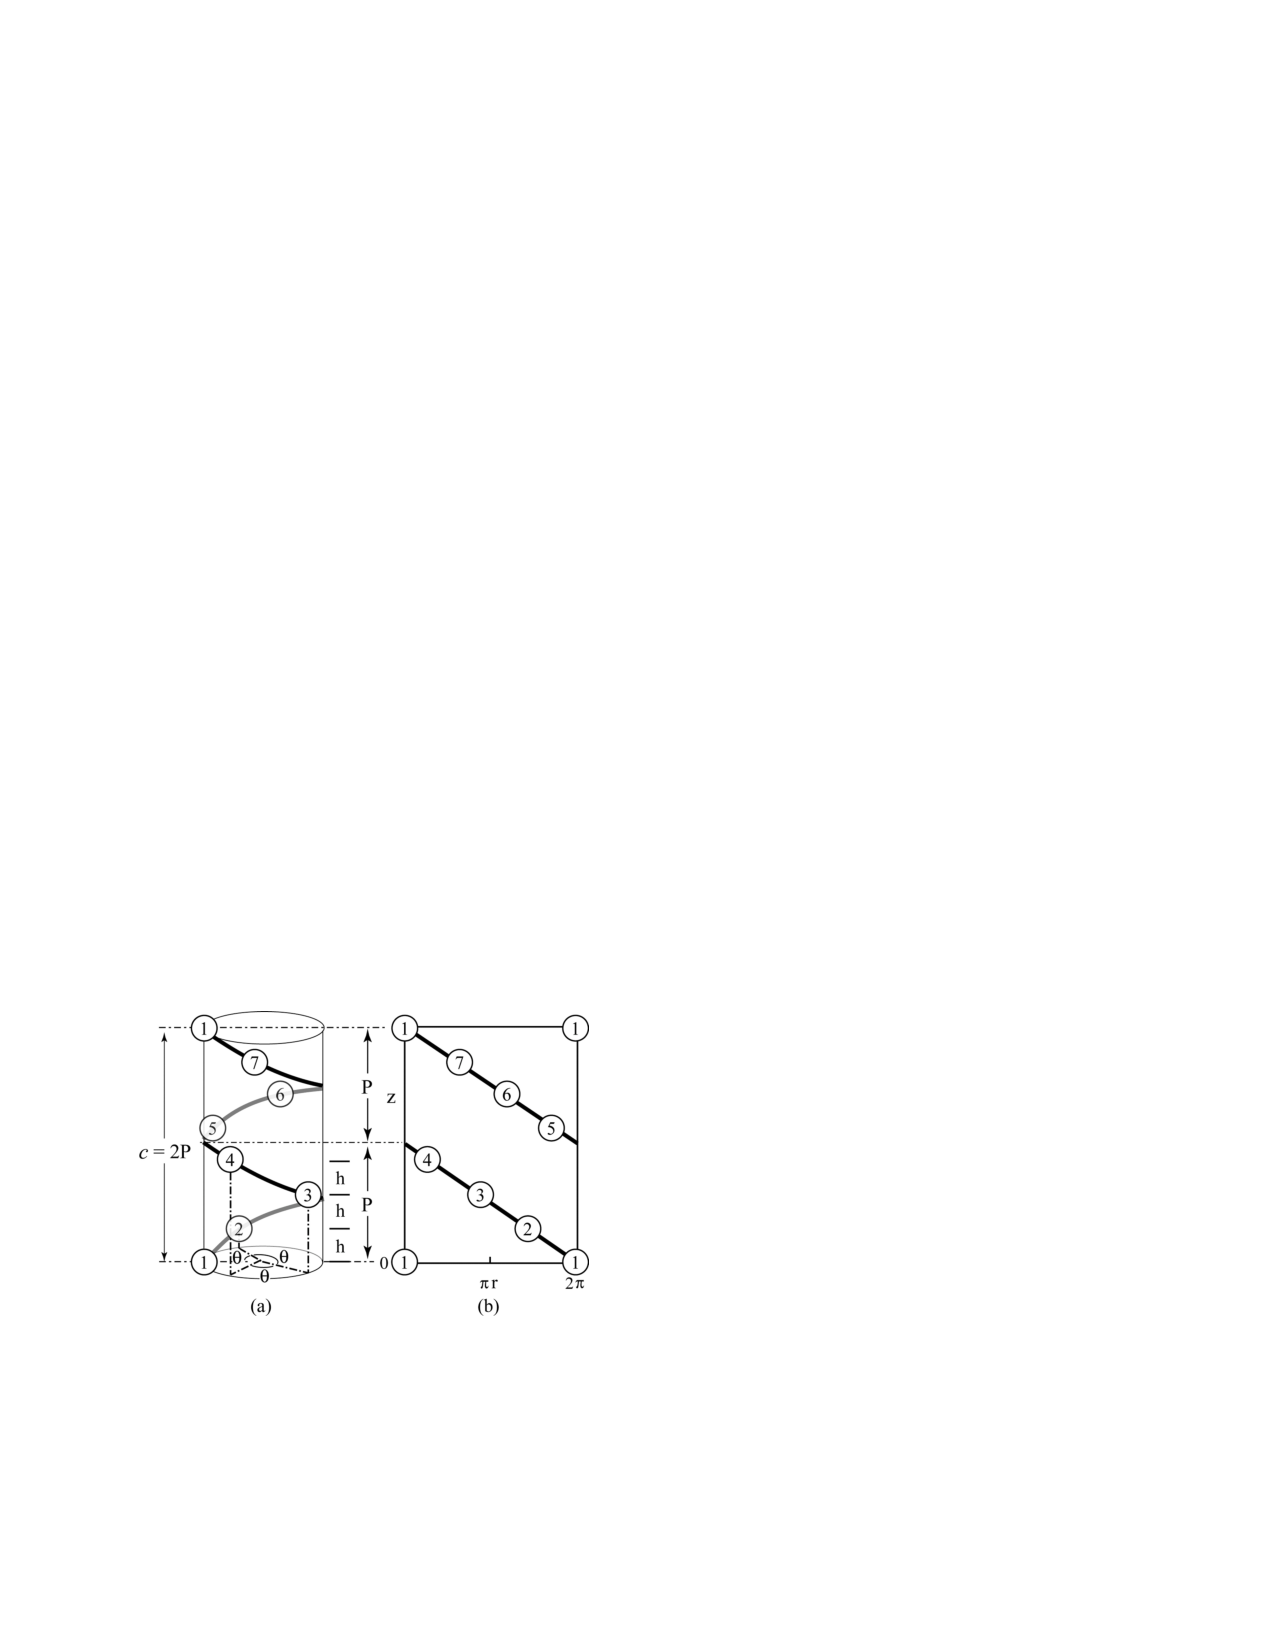
\includegraphics[width=0.7\linewidth]{helix}
\caption[7/2 helix structure (a) and its radial projection (b).]{7/2 helix structure (a) and its radial projection (b). Circles with numbers represent monomers. Pitch length, P, and unit length, h, represent the axial lengths of one helical turn and one monomer, respectively. $\theta$ represents the angle between two monomers around the helical axis, and $r$ represents the helix radius. Adopted from \cite{Okuyama2008}.}
\label{fig:PEOhelix}
\end{figure}

Low molecular weight PEO fractions, or PEO oligomers, crystallize with chains folded a small number of times, or even fully extended \cite{Kovacs1975,Kovacs1977}. The number of folds depends on many factors including crystallization temperature, chain length, cooling rate, etc. The thickness of the lamella $L$ is thus determined by the number of folds $n$ and the chain length $\lambda$:

\begin{equation}
\label{eqn_thickness}
L = \dfrac{\lambda}{1+n} = \dfrac{N l_{c}}{1+n}
\end{equation}

\noindent
where $N$ is the number of monomers in a chain, or the degree of polymerization. Especially for fully extended chains, $n = 0$, and the thickness of the lamella is equal to the chain length.

In terms of chain folding, we have also discussed about the two different chain re-entry models in \ref{folded chain model}: adjacent re-entry model and random re-entry model. In the case of PEO oligomers, the chains are relatively short, and there are not as many entanglements among the chains, so we could expect more adjacent re-entries in the lamellae.

\subsection{Melting points of PEO oligomers} \label{Tm and Yeates}

Gibbs Thomson equation (Equation \ref{eqn_GT}), enables one to build the relation between melting points and other physical parameters of a polymer crystal. In order to be consistent with other researches on PEO melting transitions, here we make some modifications to the original equation:

\begin{equation}
\label{eqn_GT2}
T_{m} = T_{m}^{\infty} (1 - \dfrac{2SV}{L \Delta H})
\end{equation}

\noindent
where $S$ is the surface free energy of the interface between the crystalline and the amorphous phase, and $V$ is the molar volume of a crystallizable repeat unit \cite{Pfefferkorn2011}. In this equation, $T_{m}^{\infty}$, $V$, and $\Delta H$ are constants that have been determined for PEO.

Melting transitions of PEO have been intensively studied through various experimental methods and from different theoretical aspects. One of the fundamental researches is of our particular interest and is worth being reviewed. Relatively monodisperse PEO oligomers with the degree of polymerization ranging from 9 to 45 were produced through step-wise syntheses by Yeates \textit{et al} \cite{Yeates1984}. Melting points of these fractions were measured, and compared to those of commercially available samples, which are much more polydisperse. Their results are shown in Figure \ref{fig:Yeates}.

\begin{figure}[H]
\center
\vspace{1 cm}
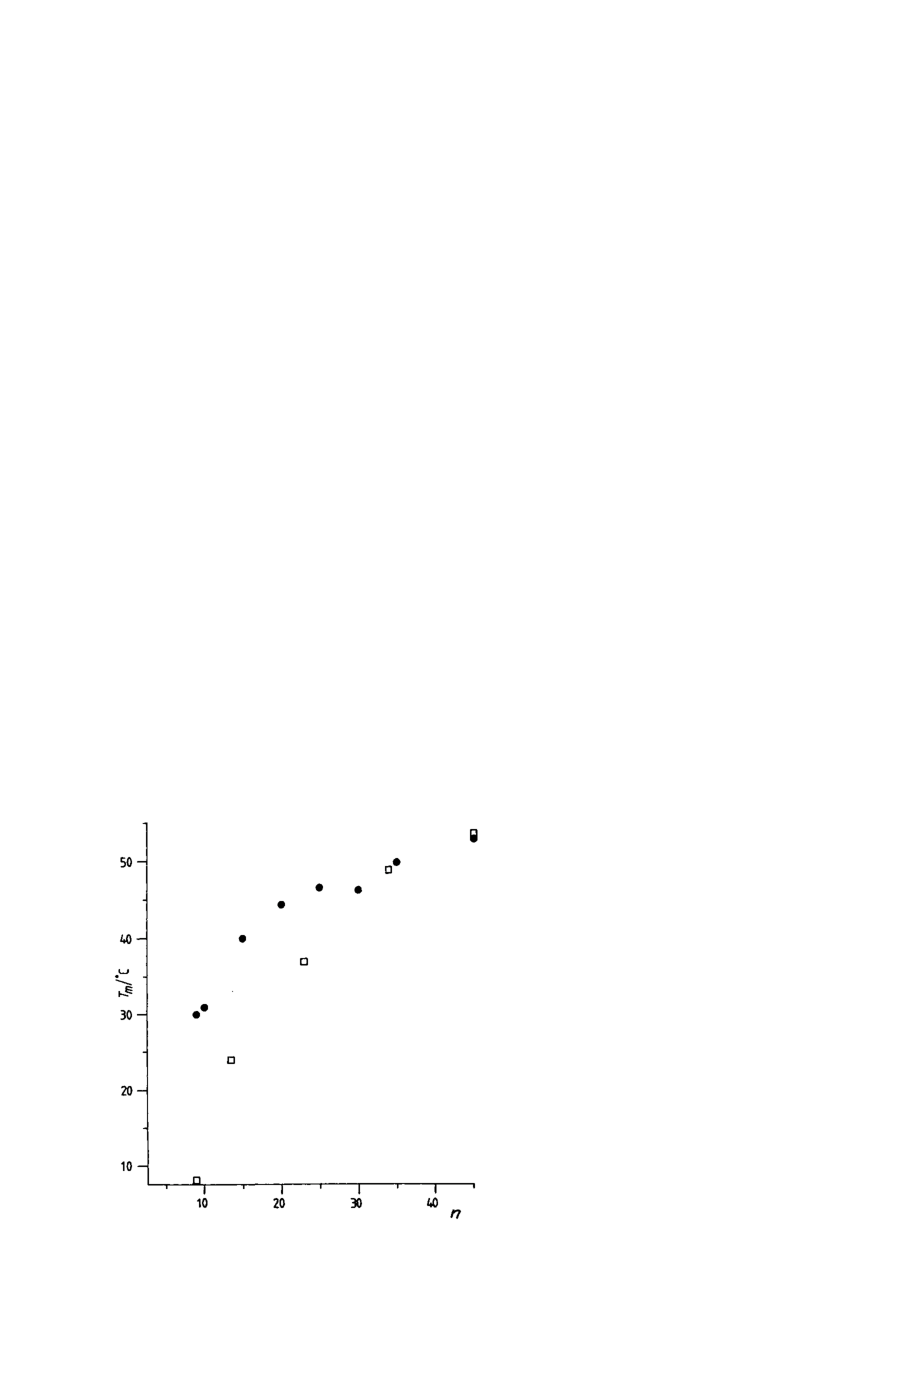
\includegraphics[width=0.5\linewidth]{Yeates}
\caption[Melting points vs degree of polymerization for monodisperse (black dots) and polydisperse (empty boxes) PEO oligomer samples.]{Melting points vs degree of polymerization for monodisperse (black dots) and polydisperse (empty boxes) PEO oligomer samples \cite{Yeates1984}.}
\label{fig:Yeates}
\end{figure}

Melting points of monodisperse samples are notably higher than those of polydisperse samples in general, and the difference is especially large for small N values. This observation indicates that polydispersity has a big influence on melting temperature, and in fact became the motivation that we conducted crystallization experiments with our purified samples, so that we could further investigate this phenomenon.

As a matter of fact, this observation has attracted much attention from researchers. One of explanations that have been proposed suggests that the $T_{m}$ difference could be related to the chain end-groups \cite{Percec1989}. In a relatively monodisperse sample, chains have roughly the same length, which makes it easier to create a smooth lamellar surface, and the end-groups would be incorporated in the crystalline array. However, in a polydisperse sample, the distribution of chains results in a more disordered lamellar surface, so some of the end-groups have to be incorporated in the amorphous phase. Because of the difference in the incorporation of chains ends, polydisperse crystals would have lower crystallinity and higher entropy, which leads to a higher melting temperature.

\section{Basics of differential scanning calorimetry}

\subsection{Phase transitions in polymers}

Phase transitions are a major aspect to study in a polymer's properties. In regular materials, phase transitions normally refer to the transitions between solid, liquid, and gaseous states. For polymer materials, we focus more on the transition between solid state and liquid state, i.e., melting transition and crystallization transition, which occur in the crystalline regions in polymers. In addition, there is a unique transition that takes place in the amorphous regions in polymers -- glass transition.

In crystalline regions, materials stay in the form of disordered melt at temperatures above $T_{m}$, and ordered crystalline solid below $T_{m}$. At melting temperature $T_{m}$, the material experiences a discontinuity in the specific volume, and absorbs or releases a certain amount of heat (depending on the direction of transition), which is called latent heat. Such transitions are classified as first-order phase transitions \cite{Jaeger1998}. 

\begin{figure}[H]
	\center
	\vspace{1 cm}
	\begin{tikzpicture}[domain=0:4] 
	\begin{axis}[
	ticks=none,
	axis x line=middle,axis y line=left,
	xlabel = {$T$},
	ylabel = {$V$},
	xmin=0,xmax=9,
	ymin=0,ymax=9,ylabel style={rotate=-90},
	]
	\addplot [mark=none] coordinates {(1,1) (5,2)};
	\addplot [mark=none, dashed] coordinates {(5,2) (5,5)};
	\addplot [mark=none] coordinates {(5,5) (8,8)};
	\addplot [mark=none, red] coordinates {(5,0) (5,2)};
	\addplot [mark=none] coordinates {(5.5,0)} node[above]{$T_{m}$};
	\addplot [mark=none] coordinates {(3,1.5)} node[above]{crystal};
	\addplot [mark=none] coordinates {(6,6.5)} node[above]{liquid};
	\end{axis}
	\end{tikzpicture}
	\caption{Temperature of specific volume of a polymer under melting or crystallization transition, where $T$ is the temperature and $V$ is the specific volume.}
	\label{fig:V vs T for Tm}
\end{figure}

In amorphous regions, materials stay in the form of disordered liquid (viscous or rubbery) at temperatures above $T_{g}$, and transform into disordered solid below $T_{g}$ \cite{InternationalOrganizationforStandardization2013}. At glass transition temperature $T_{g}$, specific volume of the material evolves continuously, and there is no latent heat involved. Such transitions are classified as second-order phase transitions \cite{Jaeger1998}. Although there is no latent heat, heat capacity of the sample does change, as indicated by the slope change in Figure \ref{fig:V vs T for Tg}. One thing to note is that glass transition normally occurs in a range of temperatures, rather than at a single point, and it always occur below $T_{m}$. This is because glass state is not a thermodynamically-stable state, and the measurement result of $T_{g}$ depends on factors such as the polymer's thermal history and the heating or cooling rate.

\begin{figure}[H]
	\center
	\vspace{1 cm}
\begin{tikzpicture}[domain=0:4] 
\begin{axis}[
ticks=none,
axis x line=middle,axis y line=left,
xlabel = {$T$},
ylabel = {$V$},
xmin=0,xmax=9,
ymin=0,ymax=9,ylabel style={rotate=-90},
]
\addplot [mark=none] coordinates {(1,2) (5,4)};
\addplot [mark=none] coordinates {(5,4) (8,8)};
\addplot [mark=none, red] coordinates {(5,0) (5,4)};
\addplot [mark=none] coordinates {(5.5,0)} node[above]{$T_{g}$};
\addplot [mark=none] coordinates {(3,3)} node[above]{glass};
\addplot [mark=none] coordinates {(6,6)} node[above]{liquid};
\end{axis}
\end{tikzpicture}
	\caption{Temperature of specific volume of a polymer under glass transition, where $T$ is the temperature and $V$ is the specific volume.}
	\label{fig:V vs T for Tg}
\end{figure}

One major difference between first-order and second-order phase transitions is their driving force. In a melting transition, the process is driven by thermodynamics, as the crystalline state is the thermodynamic ground state at low temperatures. However, the glass state is not a ground state, with the chains not being fully ordered. It has been suggested in some theoretical predictions that given long enough relaxation time, the glass state finally transform into crystalline state \cite{Gotze2009}. Instead of being thermodynamically driven, glass transition is normally considered as a kinetic transition.

\subsection{Working mechanism of differential scannign calorimetry}

The products pressed into Al pans previously are characterized with a differential scanning calorimeter (DSC) (Q100, TA Instruments). DSC is an instrument that measures the change of heat flow to the sample material within a controlled temperature range. Inside a typical DSC there are two metal (Al commonly) pans, with one acting as the sample pan and another empty pan acting as a reference. Through precise heating and cooling control with a feedback mechanism, the two pans are maintained at the same temperature at any time during the scanning measurement. At temperatures where phase transitions of the sample material takes place, the heat capacity of the sample changes, which requires the computer to adjust the amount of heat flow provided, in order to always keep the two pans at the same temperature. Heat flow $\dfrac{dQ}{dt}$ could be obtained as a function of temperature, which depends both on the heat capacity $C_{p}$ of the sample and the scanning rate $q$:
\begin{equation}
\label{eqn_DSC}
\dfrac{dQ}{dt} = \dfrac{dQ}{dT}\cdot\dfrac{dT}{dt} = C_{p} q
\end{equation}

By plotting the difference in heat flow to the two pans with respect to temperature, thermal transitions the sample material experienced during the set range of temperature, such as crystallization, melting, and glass transition, could be determined. Figure \ref{fig:DSCcurveeg} is a typical DSC curve. When the scanning rate is constant, first-order transitions appear as peaks on the DSC curve. Crystallization appears as an exothermic peak on the cooling curve, and melting appears as an endothermic peak on the heating curve. The difference observed between the crystallization temperature $T_{c}$ and the melting temperature $T_{c}$ is supercooling $\Delta T$. Note that here in this figure crystallization and melting are presented on the same curve for the sake of neatness, but they in fact occur on separare curves.

\begin{figure}[H]
\center
\vspace{1 cm}
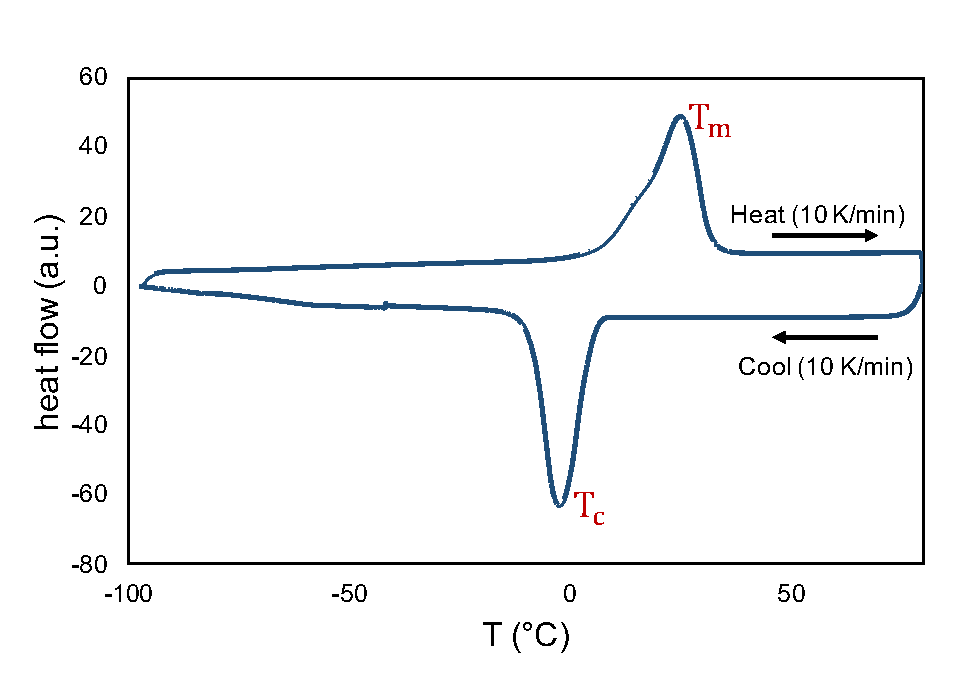
\includegraphics[width=0.6\linewidth]{DSCcurveeg}
\caption[A typical DSC curve for a polymer sample.]{A typical DSC curve for a polymer sample \cite{Misutsu2015}.}
\label{fig:DSCcurveeg}
\end{figure}

\section{Results from differential scanning calorimetry}

The following running process is performed on each product: equilibrate at 353 K (to fully melt all crystal); isothermal for 5 min; ramp 10 K/min to 173 K (to crystallize the sample); isothermal for 5 min; ramp 10 K/min to 353 K; isothermal for 5 min; ramp 10 K/min to 173 K; isothermal for 5 min; ramp 10 K/min to 353 K. With two runs of the same procedure, we examine the reproducibility of the results.

\subsection{Melting temperature}

From the DSC curves of each fraction, we determined their melting temperature, $T_{m}$, as shown in Figure \ref{fig:Tm}. Most of the samples show a double-peak pattern, with a lower $T_{m1}$ and a higher $T_{m2}$. Each measurement is carried out for more than once, and the $T_{m}$ values from separate measurements normally vary within $\pm$ 2 degrees. $\bar{N}$ is the average $N$ value of each sample, which is interpolated linearly based on the 10 samples measured with MALDI. In general, the melting temperatures behave as Gibbs Thomson relation describes, with the higher $N$ values (longer chains) showing higher melting temperatures.

\begin{figure}[H]
\center
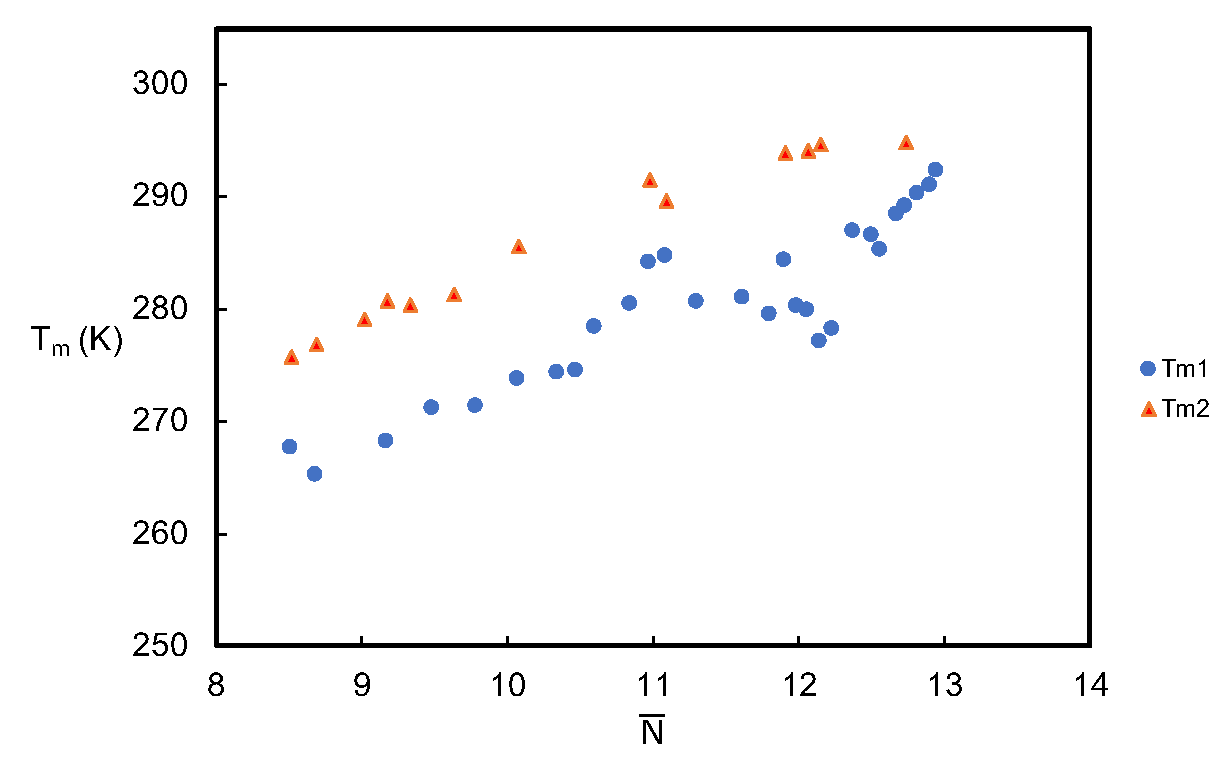
\includegraphics[width=\linewidth]{Tm}
\caption{Melting temperature of purified fractions.}
\label{fig:Tm}
\end{figure}

\subsubsection{Chain-folding analysis based on $T_{m}$}

In figure \ref{fig:Tm}, it is obviously seen that the data points potentially lie on two parallel curves, which brings our assumption that they could correspond to two types of chain-folding modes in the crystal lamellae, with the higher $T_{m}$'s being extended chains (larger thickness), and the lower $T_{m}$'s being once-folded chains (smaller thickness).

In order to validate our assumption, we apply Equation \ref{eqn_GT} to see if we are able to get a good fit with the two series of data. Parameters for PEO present in this equation, including $T_{m}^{\infty}$ \cite{Buckley1975}, $V$ \cite{Wong2015}, $\Delta H$ \cite{Yave2010} are found in the literature. Interfacial tension $S$ is dependent on the mode of chain-folding, as both chain ends and chain folds contribute to the amorphous phase, and they lead to different interfacial tensions with respect to the crystalline phase.

Interfacial tension of chain folds, $S_{folds}$, could be obtained from parameters of PEO chains with large enough molecular weights. This is because in the crystal lamellae of long chains, the number of chain folds are much greater than that of chain ends, and thus $S$ is dominated by chain folds. For long PEO chains, crystal lamellar thickness $L$ is normally on the order of 10 nm \cite{Okerberg2007}, and the melting temperature of high molecular weight PEO is around $65^\circ$C \cite{Herzberger2015}. With the other parameters previously found, we are able to calculate $S_{folds}$ from Equation \ref{eqn_GT}.

However, to quantitatively look at the thermodynamics of extended chains and once-folded chains in our assumption, and to fit  Gibbs Thomson relation of these two modes to our data, we need to know the actual interfacial tensions in these two modes. 

For extended chains, the interfacial tension $S_{ext}$ merely comes from chain ends, while for once-folded chains, apart from the chain ends, there are also chain folds that contribute to the interfacial tension $S_{1-fold}$. $S_{ext}$ and $S_{1-fold}$ could be obtained by adjusting their values based on $S_{folds}$ (previously calculated for long chains). The reason we are able to do this is that even though they arise from different parts in the polymer, interfacial tension between crystalline and amorphous regions should not vary significantly (at least on the same scale) for a certain polymer. The following two figures and illustrations are on how we achieved our fitting and established our model on the conformation of chains.

For extended chains, we fit the higher melting points with Gibbs Thomson equation, using the value of $S_{folds}$ initially, and then adjust its value until we get a good enough fit (Figure \ref{fig:fitTm1}). This value is then taken as $S_{ext}$.

\begin{figure}[H]
\center
\vspace{1 cm}
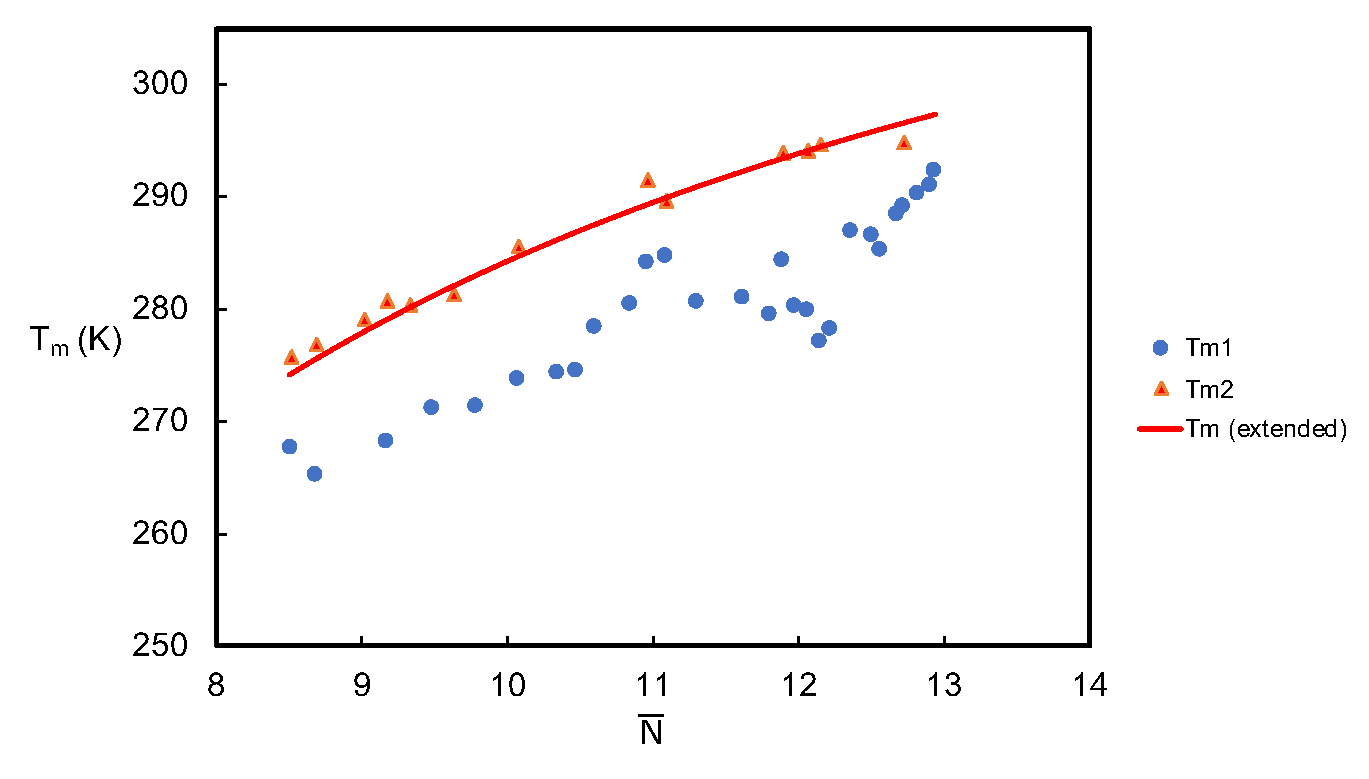
\includegraphics[width=\linewidth]{fitTm1}
\caption{$T_{m1}$ data fitting to Gibbs Thomson equation.}
\label{fig:fitTm1}
\end{figure}

For the lower melting points, which correspond to once-folded chains, the chains emanating from the lamella enter the amorphous phase to make a fold, and then re-enter the lamella. In this case we suppose that it takes $N_{a}$ monomers for a single chain to complete this turn, instead of bending $180^\circ$ sharply. This conformation has two chain-end monomers on one side of the lamella, and $N_{a}$ monomers on the fold on the other side, which enables us to calculate the interfacial tension $S_{1-fold}$ as:

\begin{equation}
\label{eqn_S1fold}
S_{1-fold} = \dfrac{2S_{ext} + N_{a} S_{folds}}{2 + N_{a}}
\end{equation}

With $S_{1-fold}$ obtained, the value of $N_{a}$ is now the only free parameter that could be tuned to fit the lower melting points with Gibbs Thomson equation. From the curve fitting (Figure \ref{fig:fitTm2}), $N_{a}$ is determined to have a value of 3.5. For a PEO chain, this is approximately 2.6 times its persistence length \cite{Takahashi1973}, which suggests that this chain conformation is a possible and reasonable model of chain-folding.

\begin{figure}[H]
\center
\vspace{1 cm}
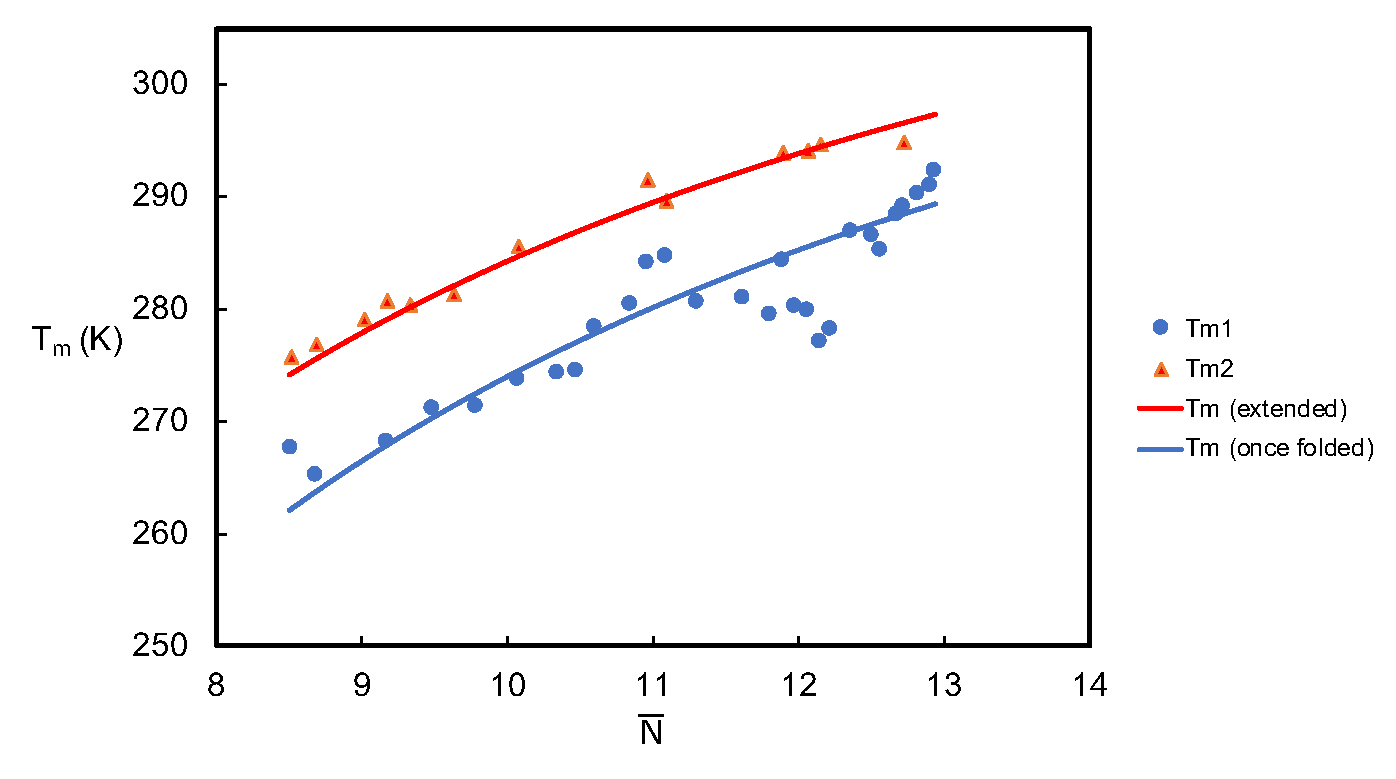
\includegraphics[width=\linewidth]{fitTm2}
\caption{$T_{m1}$ and $T_{m2}$ data fitting to Gibbs Thomson equation.}
\label{fig:fitTm2}
\end{figure}

In the plots of melting temperatures, the x-axis, $\bar{N}$, is the number average value of all the composing $N$'s in each fraction, characterized directly with MALDI or interpolated based on the MALDI data. However, only with single integer $N$ values could we be able to talk about the melting temperatures given by the Gibbs Thomson curves. For a mixtures of different $N$'s, its melting temperature potentially lies anywhere within the range of $T_{m}$'s of its composing $N$'s. A more careful way to present our chain-folding models together with the $T_{m}$ data would be as Figure \ref{fig:fitTm} shows. Dashed boxes are generated for each $T_{m}$ curve, with the top (bottom) of the box representing the melting point of the highest (lowest) $N$ value present in any potential purified fraction lying on the curve in this particular box. In generating the bars, $N$ components with a percentage less than 5 \% are neglected. Notice that each curve passes through all of the corresponding boxes, with only several data points falling outside.

\begin{figure}[H]
\center
\vspace{1 cm}
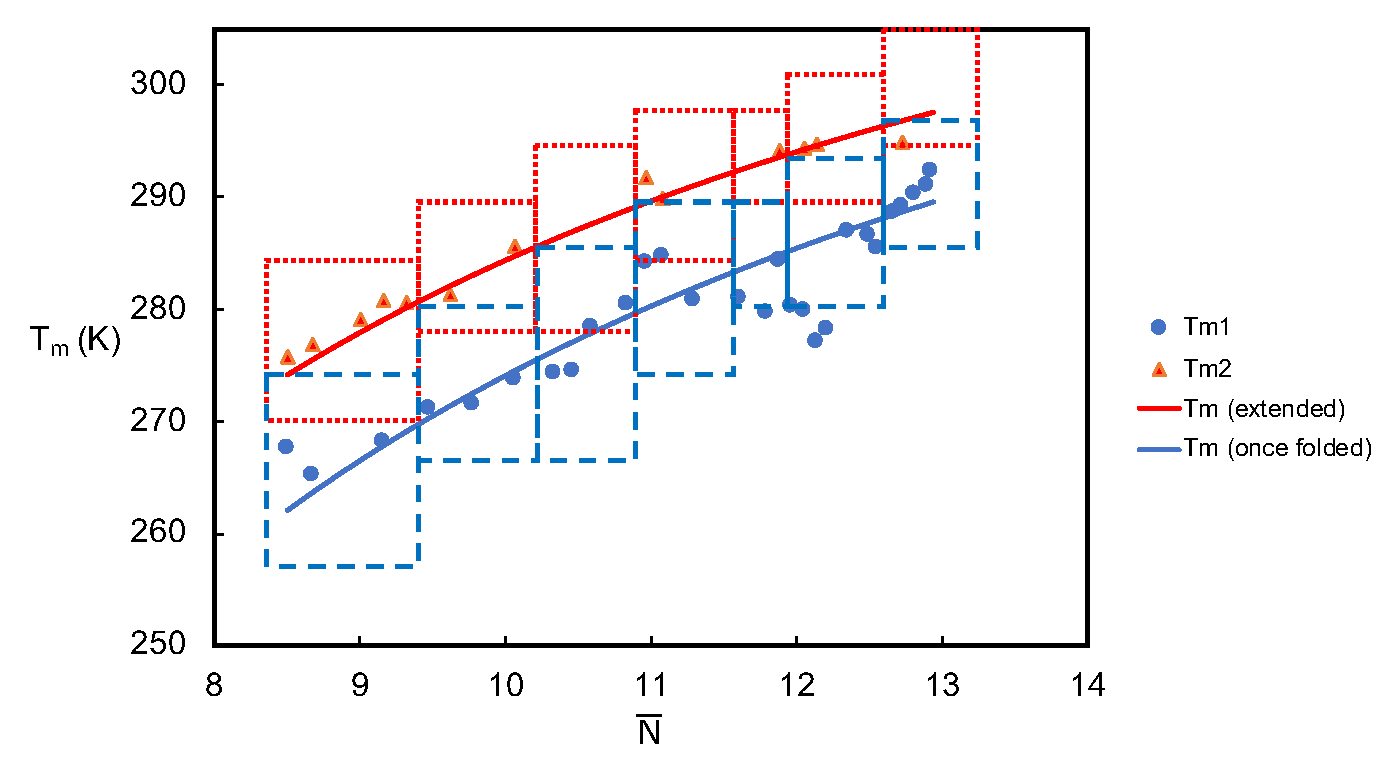
\includegraphics[width=\linewidth]{fitTm}
\caption{Gibbs Thomson relation fitting with potential range bars on $T_{m}$ data points.}
\label{fig:fitTm}
\end{figure}

In the DSC measurements, fractionation of chains with different N's is sometimes observed. During some of the repeated DSC measurements, several samples show double melting peaks (an example shown in Figure \ref{fig:3K difference}), with both melting temperatures near the same $T_{m}$ curve. The two peaks are separated by around 3 K, which is likely the difference between the melting temperatures of two neighboring N's according to our calculation, rather than the difference between the two chain conformations (extended and folded). It is worth noting that this fractionation is more commonly observed at the higher $T_{m}$ than at the lower $T_{m}$, because in the extended conformation, the crystal lamellae composing of two neighboring N's have a large difference in thickness than in the folded conformation.

\begin{figure}[H]
	\center
	\vspace{1 cm}
	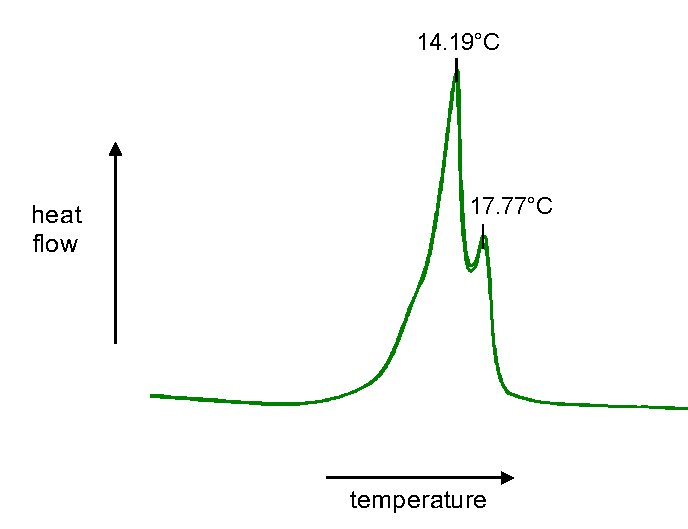
\includegraphics[width=0.5\linewidth]{doublepeaks3K}
	\caption{Part of DSC curve (melting) from regular run on $\bar{N} = 11$.}
	\label{fig:3K difference}
\end{figure}

\subsubsection{Tuning chain-folding mode}

Most of the fractions show two melting points in DSC measurements, while some of the fractions only shows one, lying either on the $T_{m1}$ curve or the $T_{m2}$ curve. For the fractions where when the higher $T_{m}$ is observed, on the DSC cooling ramp there are usually two crystallization peaks, suggesting that the polymers still form both extended chains structure and folded chains structure, but before increasing to the melting temperature, once-folded chains relax themselves and recrystallize into extended form. However, when the lower $T_{m}$ is observed, on the cooling ramp there is only one crystallization peak. This is an indication that the cooling rate during crystallization may not have been slow enough for the chains to crystallize in the extended form.

The following treatment (Figure \ref{fig:treatment}) is then applied to further verify our observation. With some of the fractions that show the lower $T_{m}$ (either with or without the higher $T_{m}$) in normal DSC measurements, we keep the sample at a temperature between $T_{m1}$ and $T_{m2}$ for a time long enough to melt all the once-folded chains and leave all the extended chains. Then we cool the sample to a much lower temperature, and measure its melting again. During the second DSC measurement only the higher $T_{m}$ appears, which is a direct validation that we have successfully forced the once-folded chains to recrystallize into extended chains by applying the treatment. Figure \ref{fig:DSC before and after} is an example measurement we did on purified fraction with $N = 12.3$.

\begin{figure}[H]
\center
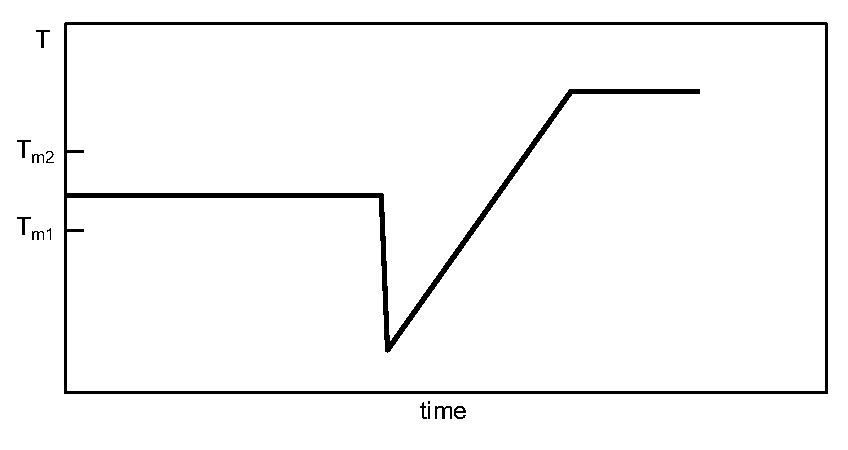
\includegraphics[width=0.6\linewidth]{treatment}
\caption{Thermal treatment on some of the products.}
\label{fig:treatment}
\end{figure}

\begin{figure}[H]
	\centering
\begin{subfigure}[b]{0.6\linewidth}
	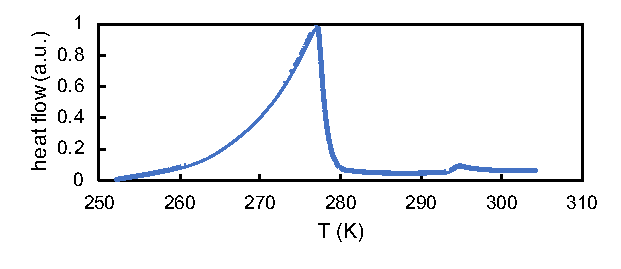
\includegraphics[width=\linewidth]{DSCbefore}
	\caption{Before thermal treatment there is a major melting transition peak followed by a small peak.}
\end{subfigure}
\begin{subfigure}[b]{0.6\linewidth}
	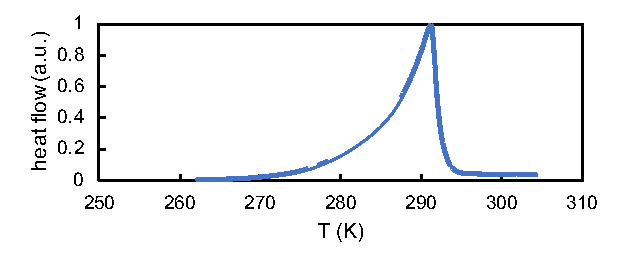
\includegraphics[width=\linewidth]{DSCafter}
	\caption{After thermal treatment only one melting peak near $T_{m2}$ is observed.}
\end{subfigure}
\caption{DSC measurements on purified fraction with $N = 12.3$ before and after thermal treatment.}
\label{fig:DSC before and after}
\end{figure}

\subsubsection{Comparison between purified fractions and neat sample}

When we compared the DSC curves of the neat sample and the purified fractions, surprisingly we noticed that some of the fractions performed unexpected melting behaviors, as Figure \ref{fig:neatvsfractions} shows. From the curves of some products from early stages of evaporation, we expect that in the neat mixed sample they should start melting at temperatures much lower than the observed melting temperature of the neat sample. However, this is not what happens. According to this phenomenon, we believe that when the short chains are mixed with longer chains, they become influenced and perform different crystallization behaviors than in a more monodisperse sample. One of the possible explanations to this is that in the presence of longer chains, the shorter chains tend to act as amorphous phase, even at temperatures lower than the melting points of themselves. As a matter of fact, it is also possible that the short chains only take up a very small portion in the neat sample, therefore the heat flow signal from them could easily be overwhelmed by that of major components.

\begin{figure}[H]
\center
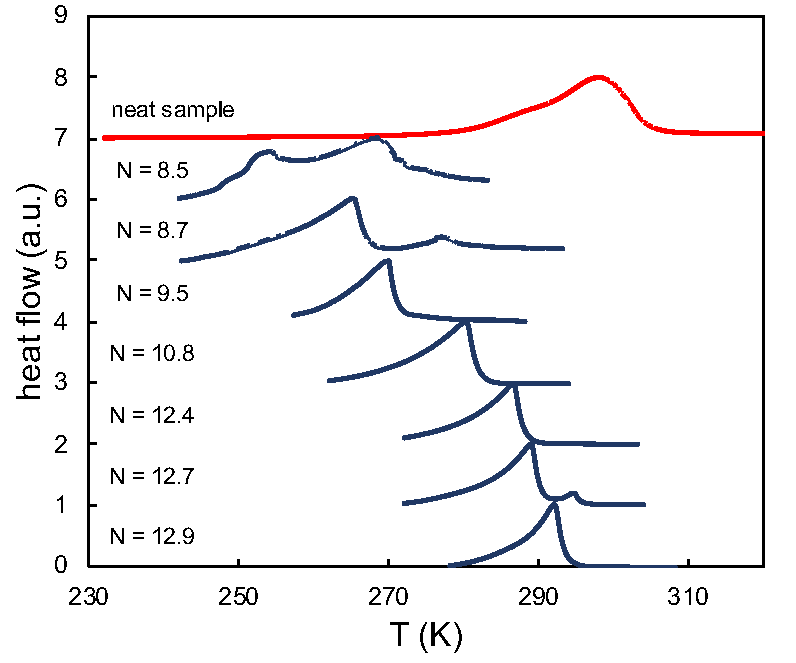
\includegraphics[width=0.8\linewidth]{neatvsfractions}
\caption{DSC curves of the neat sample (red) and some of the purified fractions (blue).}
\label{fig:neatvsfractions}
\end{figure}

\subsubsection{End-group effects}

In \ref{Tm and Yeates}, we reviewed Yeates' study on melting of monodisperse and polydisperse PEO oligomers. Now we would like to compare our results for purified fractions with theirs. Surprisingly, it turns out that the melting temperatures we obtained agree more with the polydisperse samples in their measurements. This could be an indication that the melting points difference they observed between the monodisperse and polydisperse samples is very unlikely to be due to polydispersity. Instead, it could be related to specific properties such as end-group chemistry.

End-group effects on PEO crystallization has been studied by many researchers and it has been found that the type of end-groups directly influences properties including melting temperature and crystallinity, as shown in Table \ref{tab:end-group effects}. Monodisperse PEO with hydroxy end-groups has been reported to display different crystallinities and $T_{m}$'s than that with methoxy end-groups. The difference in crystallinity is believed to be due to different heats of interaction related to the end-groups at the lamellar surfaces. The difference in melting temperature is attributed to different environments at a crystalline lamellar surface and in melt, because lamellar surfaces are much more ordered compared to the melt, which magnifies the effect of end-groups on the surfaces, while in a melt environment, the effect of end-groups could be hidden in the melt background. Polydisperse PEO samples with different end-groups, however, display different crystallinities but similar $T_{m}$'s. It is argued that rejection of methoxy end-groups from the lamellar surfaces results in higher entropy of the crystal, leading to a lower enthalpy of melting, and a lower crystallinity. In terms of the melting temperature, it is claimed that the disordered lamellar surface and the melt have similar environments, so the effect of end-groups on $T_{m}$'s would appear less significant.
\begin{table}[H]
\centering
	\begin{tabular}{ |c|c|c|c| } 
		\hline
		 & monodisperse PEO & polydisperse PEO \\
		\hline
		\hline
		crystallinity & different & different \\ 
		\hline
		$T_{m}$ & different & similar \\ 
		\hline
	\end{tabular}
	\caption{\label{tab:end-group effects}Comparison of PEO with hydroxy and methoxy end-groups \cite{Marshall1981}.}
\end{table}
In our experiments, the PEO samples only contain hydroxy end-groups, while in Yeates' study, the synthesis of monodisperse samples involved end-groups containing sulfur. Based on the evidences and analysis mentioned above, the  disagreement between our results and theirs could be that sulfur results in different interaction energy with the crystalline layer, and potentially led to different melting temperatures. From literature it is found that sulfur decreases the interfacial tension of liquid iron with $\text{Al}_{\text{2}}\text{O}_{\text{3}}$ \cite{Halden1955}, and also decreases the interfacial energy between Fe-C melt and graphite \cite{Jung2005}. However, no direct measurement results have been found in terms of the effect of sulfur-containing end-groups on the interfacial energy and melting temperature of a polymer.

\subsection{Degree of crystallinity}

PEO has been know as a polymer with high crystallinity due to its linear structure. However, based on the fact that polymers almost never crystallizes completely, it is of interest to study the degree of crystallinity $X_{c}$ of our samples. We determine $X_{c}$ of the products from the heat of fusion $\Delta H_{f} (T_{m})$ on melting in DSC measurements. The heat of fusion could be calculated from the area under the melting peak, and the degree of crystallinity is defined as \cite{Kong2002}:

\begin{equation}
\label{eqn_Xc}
X_{c} = \dfrac{\Delta H_{f} (T_{m})}{\Delta H_{f}^{0} (T_{m}^{0})}
\end{equation}

\noindent
where $X_{c}$ is the degree of crystallinity by weight fraction, $\Delta H_{f} (T_{m})$ is the enthalpy of melting transition, and $\Delta H_{f}^{0} (T_{m}^{0})$ is the enthalpy of melting of PEO with 100 \% crystallinity \cite{Yave2010}. By integrating the melting peaks on the DSC curves, we obtain $X_{c}$ of the purified products, as shown in Figure \ref{fig:Xc}.

\begin{figure}[H]
\center
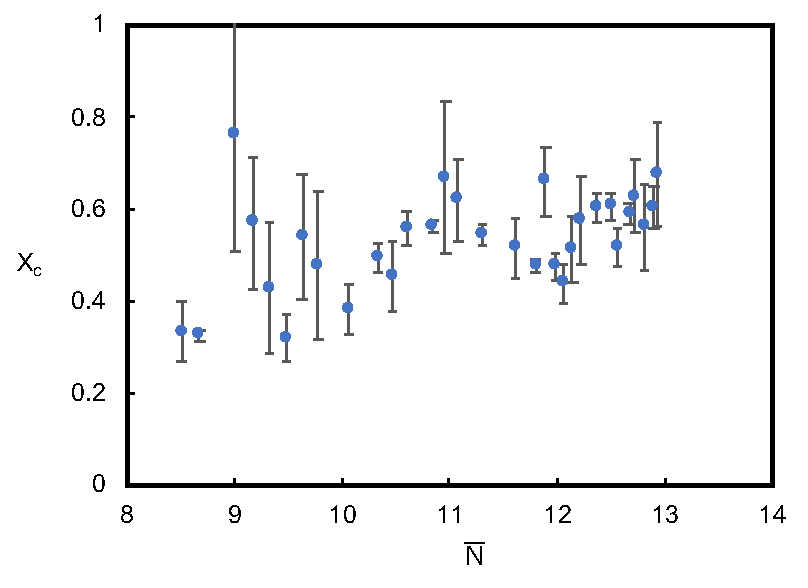
\includegraphics[width=0.7\linewidth]{Xc}
\caption{Degree of crystallinity of purified products.}
\label{fig:Xc}
\end{figure}

It is easily noticed from the figure that our data is not precise enough since the error bars for some of the fractions are quite large. This results from the deviation (0.1 mg) of the scale used to weigh the samples. The enthalpy of melting $\Delta H_{f} (T_{m})$ calculated from the DSC curve is directly related to the weight of sample, and for samples with a small weight, the deviation is comparable to its weight. Therefore, for more precise data of $X_{c}$, larger amount of sample is required, which brings forward the demand for technical improvements including scaling-up of our evaporative purification system.

We would also like to compare our results of PEO crystallinity with other studies, as shown in Figure \ref{fig:Xc comparison}. Although there is a limited number of measurement results on PEO crystallinity with such low $\bar{N}$ values, most of our results lie in the range of several other studies in the literature.

\begin{figure}[H]
	\center
	\vspace{1 cm}
	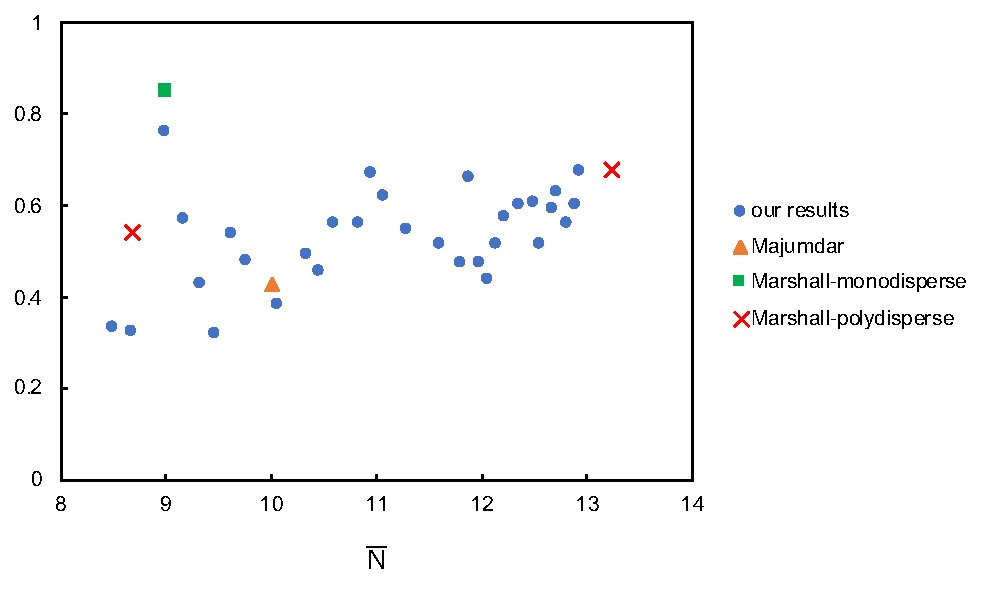
\includegraphics[width=0.9\linewidth]{Xccomparison}
	\caption[Comparison of degree of crystallinity measured in different studies]{Comparison of degree of crystallinity measured in different studies \cite{Majumdar2010}\cite{Marshall1981}.}
	\label{fig:Xc comparison}
\end{figure}

An interesting fact about the $X_{c}$ data is that when we bring Figure \ref{fig:Xc} and Figure \ref{fig:Tm} into comparison (even though $X_{c}$ and $T_{m}$ are not directly related), it could be noticed that they have a similar trend, especially with the bump pattern located at $\bar{N}$ around 11. However, the reason behind this observation is still unclear to us and needs further investigation.